\documentclass[12pt]{article}
\usepackage{graphicx}
\usepackage[margin=25mm]{geometry}
\usepackage{amsmath}
\usepackage{amssymb}
\usepackage{biblatex}
\usepackage{booktabs}
\usepackage{float}
\usepackage{tabularx}
\renewcommand{\thesubsection}{(\alph{subsection})}
\begin{document}

% Cover Page
\pagebreak
\begin{titlepage}
    \begin{center}
        \vspace*{\fill}
        Lab 6: The $e/m$ Ratio for Electrons

        Author: Shaaz Feerasta

        CCID: feerasta

        Student ID: 1704756

        Lab Partner(s): Morgann Reinhart

        PHYS 126, LAB HR81

        TA: Nicolas Concha Marroquin

        Date of Lab: March 6, 2025
        \vspace*{\fill}
    \end{center}
\end{titlepage}

\section{Linearization}
We start with our force balance equation:
\begin{align*}
    evB_{\perp} &= \frac{mv^2}{r} \\
    B_H - B_E &= \frac{mv^2}{evr} \\
    \text{From conservation of energy: } v &= \sqrt{\frac{2eV}{m}} \\
    \therefore B_H &= \frac{m\left(\frac{2eV}{m}\right)}{er\sqrt{\frac{2eV}{m}}} + B_E \\
    B_H &= \frac{2V}{r\sqrt{2eV/m}} + B_E\\
    B_H &= \sqrt{\frac{m}{e}}\frac{\sqrt{2V}}{r} + B_E \\
    \therefore \frac{8\mu_0NI}{\sqrt{125}R} &= \sqrt{\frac{m}{e}}\frac{\sqrt{2V}}{r} + B_E
\end{align*}
Then, for $y = mx + b$: \\
$y = B_H$, $m = \sqrt{m/e}$, $x = \sqrt{2V}/r$, and $b = B_E$

\section{Background Magnetic Field}
There are two main sources of magnetic field within the laboratory actually. There is also Earth's magnetic field as well,
the cool thing that makes a compass work.
\section{Earth's Magnetic Field}
When using LINEST, we find our $B_E$ $\approx 2.34 \times 10^{-8}$ T.
When comparing our $B_E$ to the Earth's magnetic field in Edmonton according to NOAA ($56.4 \times 10^{-6}$), we can see that
the NOAA value is much larger. More specifically, $\frac{56.4 \times 10^{-6}}{2.34 \times 10^{-8}} \approx 2410$ times larger.
\\ \\
\noindent When calculating our Helmholtz magnetic field strength with $I = 0.00313$ A:
\begin{align*}
    B_H = \frac{8}{\sqrt{125}R}\mu_0NI = \frac{8}{(0.33)\sqrt{125}}(1.25663706212 \times 10^{-6})(72)(0.00313) \approx 6.13 \times 10^{-7}\text{ T}
\end{align*}
When dividing the two, we end up getting: $\frac{6.13 \times 10^{-7}}{56.4 \times 10^{-6}} \approx 0.001$, and so, our Helmholtz magnetic
field strength is approximately 0.001 times larger than the Earth's magentic field
\section{Helmholtz Orientation}
The Helmholtz coils are oriented exactly 18 degrees to help negate the effect of Earth's magnetic fields. This helps
us to conduct our experiment in a controlled manner without any external forces (or fields) impacting our results.
\section{Magnetic Field Direction}
When viewing our experiment from a top-down view, our magnetic field direction would be going OUT of the page, or in real life, it would be going towards
the roof of the building. We know this because of the right-hand rule. Our forefinger goes to the direction a positive charge would be going, so down.
Then, our thumb, when directly perpendicular to the forefinger, goes towards the force, which is to the right of the page.
Finally as a result, our palm is facing into the page. However, we need to remember that this is the case of a positive charge, so the electron would be opposite, and so
would be coming OUT of the page., and so our final answer is out of the page.
\section{Table}
\begin{table}[H]
    \centering
    \caption{Raw experimental data along with the data used to plot our values (the last two columns). Note that the values were calculated using SI values of our measured data.}
    \begin{tabularx}{\textwidth}{X X X X X X}
        \toprule
        \text{Current (mA)} & \text{Diameter (cm)} & \text{Voltage (V)} & \text{$B_H$ ($\times 10^{-7}$ T)} & \text{$\sqrt{2V}/r$} \\
        \midrule
        1.43 & 11.5 & 25 & $2.8 \pm 0.1$ & $123 \pm 1$ \\
        2.01 & 10.3 & 25 & $3.9 \pm 0.1$ & $137 \pm 2$ \\
        2.26 & 9.00 & 25 & $4.4 \pm 0.1$ & $157 \pm 2$ \\
        2.62 & 7.80 & 25 & $5.1 \pm 0.2$ & $181 \pm 2$ \\
        3.13 & 6.50 & 25 & $6.1 \pm 0.2$ & $218 \pm 3$ \\
        1.96 & 11.5 & 30 & $3.8 \pm 0.1$ & $135 \pm 1$ \\
        2.18 & 10.3 & 30 & $4.2 \pm 0.1$ & $150 \pm 1$ \\
        2.45 & 9.00 & 30 & $4.8 \pm 0.2$ & $172 \pm 2$ \\
        2.78 & 7.80 & 30 & $5.5 \pm 0.2$ & $199 \pm 2$ \\
        3.22 & 6.50 & 30 & $6.3 \pm 0.2$ & $238 \pm 3$ \\
        2.14 & 11.5 & 35 & $4.2 \pm 0.1$ & $146 \pm 1$ \\
        2.36 & 10.3 & 35 & $4.6 \pm 0.2$ & $162 \pm 1$ \\
        2.62 & 9.00 & 35 & $5.1 \pm 0.2$ & $186 \pm 2$ \\
        2.98 & 7.80 & 35 & $5.9 \pm 0.2$ & $215 \pm 2$ \\
        3.47 & 6.50 & 35 & $6.8 \pm 0.2$ & $257 \pm 3$ \\
        \bottomrule
    \end{tabularx}
    \label{tab:experimental_data}
\end{table}

\section{Graph}
\begin{figure}[H]
    \centering
    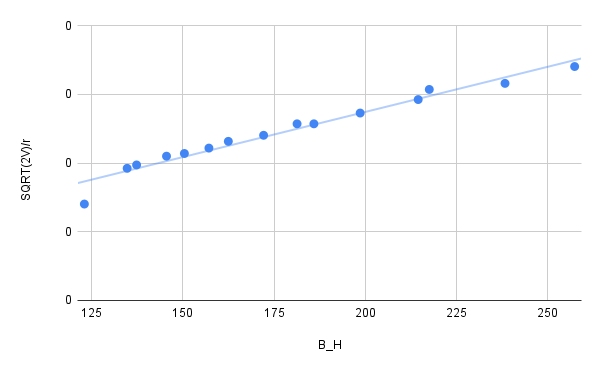
\includegraphics[width=\textwidth]{chart.png}
    \caption{Graph of $B_H = \sqrt{\frac{m}{e}}\sqrt{2V}/r + B_E$, with slope $\sqrt{m/e} = (2.6 \pm 0.1) \times 10^{-9}$ kg/J and intercept $B_E = (3 \pm 3) \times 10^{-8}$ T.
        We used this to find our e/m ratio.}
    \label{fig:bh_vs_sqrt2v_r}
\end{figure}
\section{E/M}
So we know our slope is $\sqrt{m/e} = (2.6 \pm 0.1) \times 10^{-9}$, so to find our $e/m$ ration,
we first square our value and then take the inverse. Our resulting value is:
\begin{equation*}
    \frac{e}{m} = \left(\sqrt{\frac{m}{e}}\right)^{-2}\approx (1.5 \pm 0.1) \times 10^{17} J/kg
\end{equation*}
\section{Comparison}
The currently accepted value for the $e/m$ ratio is $\frac{1.602176634 \times 10^{-19}}{9.1093837015 \times 10^{-31}} \approx 1.76 \times 10^{11} J/kg$.
Although, we can easily see that compared to our measured value, the accepted $e/m$ ratio is greater than three error intervals away from our experimental value.
i.e;
\begin{equation*}
    3\delta\left[\left(\frac{e}{m}\right)_{experimental} - \left(\frac{e}{m}\right)_{accepted}\right] < \left(\frac{e}{m}\right)_{experimental} - \left(\frac{e}{m}\right)_{accepted}
\end{equation*} 
And so we can conclude that the numbers do not agree.
\renewcommand{\bibname}{5\ \ \References and Acknowledgements}
\begin{thebibliography}{9}
    \bibitem{labmanual} 
    Department of Physics. \textit{PHYS 126 Lab Manual}. University of Alberta, 2025.

    \bibitem{person}
    TA assisted with the lab, and provided guidance on the data collection and analysis.

    \bibitem{person}
    Lab partner Morgann Reinhart assisted with the data collection and analysis.
    
\end{thebibliography}

\end{document}
